\documentclass[12pt, a4paper, english]{report}
\usepackage[utf8]{inputenc}
\usepackage{makecell}
\usepackage{fourier}
\usepackage{caption}
\usepackage{amssymb}
\usepackage[linesnumbered]{algorithm2e} %,lined,boxed,commentsnumbered
\usepackage{subcaption}
\usepackage{epigraph}
\usepackage{tikz}
\usepackage{babel}
\usepackage{amsfonts}
\usepackage{geometry}
\usepackage{hyperref}
\usepackage{csquotes}
\usepackage{underscore}
\usepackage{amsmath}
\usepackage{amsthm}
\usepackage{thmtools}
\usepackage{biblatex}
\usepackage[rightcaption]{sidecap}
\usepackage{graphicx}
\usepackage{tabularx}

\SetKwComment{Comment}{/*}{*/}
\SetKw{GoTo}{GoTo}
\SetKwData{List}{List}
\SetKwFunction{Append}{append}

\newtheorem{theorem}{Theorem}
\newtheorem{definition}{Definition}
\newtheorem{lemma}{Lemma}

\DeclareMathOperator*{\argmin}{arg\,min}

\graphicspath{ {img/} }

\author{Niccolò Simonato}
\title{Cryptography: notes}

\begin{document}

\maketitle

\tableofcontents

\chapter{Elements of Number Theory}
\section{Definitions of Number Theory}
\subsection{The cyclic group $\mathbb{Z}_{n}^{*}$}
The cyclic group $\mathbb{Z}_{n}^{*}$ is defined as
\[
\mathbb{Z}_{n}^{*} = \{a \in \mathbb{Z}_{n}: (a,n) = 1\}
\]
The \textbf{generator} of $\mathbb{Z}_{n}^{*}$ is a number in $\mathbb{Z}_{n}^{*}$ such that:
\[
\forall a \in \mathbb{Z}_{n}^{*}: \exists i: a \equiv_{m} g^{i}
\]
For this reason, $\mathbb{Z}_{n}^{*}$ is also referred as $< g >$.\newline
An interesting property is that only for $[1,2,4, \phi, \phi^{\alpha}, 2 \phi^{\alpha}]$,
 $\mathbb{Z}_{n}^{*}$ is cyclic, where $\phi$ is a prime number and $\phi^{\alpha}$ is a power of a prime number.\newline

\subsection{Pseudoprime number}
For an integer $a > 1$, if a composite integer $x$ divides $a^{x-1} - 1$, then $x$ is called a \textbf{Fermat pseudoprime} to base $a$.
\[
x \text{ is spsp(a) } \iff x|a^{x - 1} - 1
\]
In other words, a composite integer is a Fermat pseudoprime to base a if it successfully passes the Fermat primality test for the base $a$.\newline
$x$ is $spsp(a)$ is a predicate, that means that some $x$ is a \emph{strong pseudoprime number in base $a$}.

\subsection{Carmichael numbers}
Carmichael numbers are defined as follows:
\begin{itemize}
    \item Let $n$ be a composite number;
    \item Then:
    \[b^{n} \equiv_{n} b \implies b \text{ is a \textbf{Carmichael number}}\]
\end{itemize}

\section{Reminders of Modular Arithmetic}
\subsection{Little Fermat's Theorem}\label{little_fermat_th}
\begin{theorem}[Little Fermat's Theorem]
    Consider what follows:
    \begin{itemize}
        \item Let $p$ be a prime number and $p \nmid a$.
        \item Then \[a^{p-1} \equiv_{p} 1\]
    \end{itemize}
\end{theorem}
\begin{proof}
    Consider what follows:
    \begin{itemize}
        \item Let's consider: \[A = \{na \bmod p: n \in [1, p-1]\}\]
        \item $A$ has all distinct elements due to the Bijection Lemma (Lemma~\ref{bijection_lemma}).
        \item Then \[A = \mathbb{Z}_{n}^{*}\]
        \item Then, \[\prod\limits_{n \in A} n \equiv_{p} \prod\limits_{n=1}^{p-1} na \implies (p-1)! \equiv_{p} (p-1)!a^{p-1}\]
        \item Therefore, $a^{p-1} \equiv_{p} 1$ for the Wilson's Theorem~\ref{wilson_th}.
    \end{itemize}
\end{proof}

\subsection{Wilson's Theorem}\label{wilson_th}
\begin{theorem}[Wilson's Theorem]
    Consider what follows:
    \begin{itemize}
        \item Let $n \in \mathbb{N} \setminus \{0,1\}$
        \item Then, \[(n-1)! \equiv_{n} -1\]
    \end{itemize}
\end{theorem}
\begin{proof}
    The proof is \textbf{by induction} on $n$:
    \begin{itemize}
        \item \textbf{Base case}: $n = 2$
        \[1! \equiv_{2} -1\]
        \item \textbf{Inductive step}:
        The theorem is assumed to be true up until $n - 1$. Let's consider the case of $n$:
        \begin{itemize}
            \item Consider the polynomial \[g(x) = (x-1)(x-2) \dots (x - (n-1))\]
            \item $g$ has degree $p-1$ and costant term $(p-1)!$. It's roots are in $[1,p-1]$.
            \item Consider \[h(x) = x^{p-1} - 1\] $h$ has also degree $p-1$ and leading term $x^{p-1}$.
            \item Let $f(x) = g(x) - h(x)$.
            \item Then, $f$ has degree at most $p - 2$ (since the leading terms cancel), and modulo $p$ also has the $n - 1$ roots $1, 2, ..., n - 1$.
            \item But Lagrange's theorem says it cannot have more than $p - 2$ roots.
            \item \[\therefore f \equiv_{n} 0\]
            \item Its costant term, \[(n-1)! + 1 \equiv_{n} 0 \iff (n-1)! \equiv_{n} -1\]
        \end{itemize}
    \end{itemize}
\end{proof}

\subsection{Euler-Fermat's Theorem}\label{euler_fermat_th}
\begin{theorem}[Euler-Fermat's Theorem]
    Consider what follows:
    \begin{itemize}
        \item Let $n \in \mathbb{Z}$ be a number.
        \item Then, \[a^{\varphi(n)} \equiv_{n} 1\]
    \end{itemize}
\end{theorem}

\subsection{Bézout's identity}
\begin{theorem}[Bezout's identity]
    Consider what follows:
    \begin{itemize}
        \item Let $a$ and $b$ be integers with greatest common divisor $d$.
        \item Then there exist integers $x$ and $y$ such that $ax + by = d$.
        \item Moreover, the integers of the form $az + bt$ are exactly the multiples of $d$.
    \end{itemize}
\end{theorem}

\subsection{Chinese Reminder's Theorem}
\begin{theorem}[Chinese Reminder's Theorem]
    Given a system of congruences:
    \begin{align*}
        x & \equiv_{m_{1}} a_{1} \\
        x & \equiv_{m_{2}} a_{2} \\
        &\dots \\
        x & \equiv_{m_{r}} a_{r}
    \end{align*}
    In which each module is prime with each others, that is:
    \[
    \forall i \neq j: (m_{i}, m_{j}) = 1
    \]
    then \textbf{there exists a simultaneous solution $x$ to all of the congruences}, and \textbf{any two solutions are congruent to one another modulo}.
    \[M = m_{1}m_{2}\dots m_{r}\]
\end{theorem}

\begin{proof}
    Consider what follows:
    \begin{itemize}
        \item Suppose that $x'$ and $x"$ are two solutions.
        \item Let $x = x' - x''$.
        \item Then x must be congruent to $0$ modulo each $m_{i}$ and hence modulo $M$.
        \item Let $M_{i} = \frac{M}{m_{i}}$, to be the product of all of the moduli except for the i-th.
        \item Then $GCD(m_{i}, M_{i}) = 1$ and therefore $\exists N_{i}: M_{i}N_{i} \equiv_{m_{i}} 1$.
        \item Set $x = \sum_{i}a_{i}M_{i}N_{i}$;
        \item Then, for each $i$ we see that the terms in the sum other than the i-th term are all divisible by $m_{i}$, because $m_{i} | M_{j}$ when $i \neq j$.
        \item Thus, for each $i$ we have: $x \equiv_{m_{i}} a_{i}M_{i}N_{i} \equiv_{m_{i}} a_{i}$,
    \end{itemize}
\end{proof}

\subsection{Bijection of a modular function Lemma}
\begin{lemma}[Bijection of a modular function Lemma]\label{bijection_lemma}
    Consider:
    \begin{itemize}
        \item \[a \in \mathbb{Z}_{n}^{*}\]
        \item \[f: \mathbb{Z}_{n} \rightarrow \mathbb{Z}_{n}\]
    \end{itemize}
    Then, $f$ is a bijection.\newline
\end{lemma}
\begin{proof}
    Part 1: $f$ is injective.
    \begin{itemize}
        \item Assume $f(x_{1}) = f(x_{2}) \in \mathbb{Z}_{n} \iff ax_{1} \equiv_{n} ax_{2}$.
        \item Then $\exists k \in \mathbb{Z}: ax_{1} - ax_{2} = kn$.
        \item Therefore,
        \begin{align*}
            a(x_{1} - x_{2}) = kn & \iff a^{-1}a(x_{1} - x_{2}) = a^{-1}kn\\
            \iff (x_{1} - x_{2}) = a^{-1}kn & \iff x_{1} - x_{2} \equiv_{m} 0.
        \end{align*}
        \item $\therefore x_{1} \equiv_{m} x_{2}$, so $f$ is an injection.
    \end{itemize}
    Part 2: $f$ is surjective.
    \begin{itemize}
        \item Let $b \in \mathbb{Z}_{n}$.
        \item Let $\overline{x} = a^{-1}b \in \mathbb{Z}_{n}$.
        \item Then, $f(\overline{x}) \equiv_{m} a \cdot \overline{x}$\\
        $\equiv_{m} a \cdot a^{-1} \cdot b \equiv_{m} b$.
        \item Therefore, $f$ is surjective.
    \end{itemize}
    Since $f$ is injective $\land$ $f$ is surjective, then $f$ is bijective.
\end{proof}

\subsection{Euler's $\varphi$ function Lemmas}
\begin{lemma}[Sum of the prime divisors' $\varphi$-function]
    \[\forall n \in \mathbb{N} \backslash \{0\}: \sum_{\frac{n}{d}} \varphi(d) = n\]
    Where $\frac{n}{d}$ is the set of prime divisors of $n$.\newline
\end{lemma}
\begin{proof}
    The proof is by \textbf{contradiction}:
    \begin{itemize}
        \item Let $B$ be \[\{\frac{h}{n}: h \in \mathbb{Z}_{n} \land n \in \mathbb{N} \}\]
        \item Therefore, \[B = \cup_{\frac{n}{d}}\{a \in \{1, \dots, n\} \land (a,d) = 1\}\]
        \item Then, \[n = |B| = \sum_{\frac{d}{n}} \varphi(d)\]
        \item Consider \[(a_{1}, d_{1}) = 1 \land (a_{2}, d_{2}) = 1 \text{, where} d_{1}|n \land d_{2}|n\]
        \item Then, \[\frac{a_{1}}{d_{1}} = \frac{a_{2}}{d_{2}} \iff a_{1}d_{2} = a_{2}d_{1}\]
        \item Then, \[d_{1}|a_{1}d_{2} \implies d_{1}|d_{2} \land
        d_{2}|a_{2}d_{1} \implies d_{2}|d_{1}\]
        \item Therefore,  $d_{1} = d_{2}$. This is clearly a \emph{contradiction}, because in $B$ each divisor is counted once.
    \end{itemize}
\end{proof}

\begin{lemma}[Number of divisors of a prime number's power]
    Let $p \in \mathbb{N}$  be a prime number, and $\alpha \in \mathbb{N}$.\\
    Then, \[\varphi(p^{\alpha}) = p^{\alpha - 1}(p - 1)\]
\end{lemma}
\begin{proof}
    The proof is by \textbf{induction} on $\alpha$.\newline
    \textbf{Case base:} $\alpha = 1$
    \[p = \sum_{\frac{d}{p}} \varphi(d) = \varphi(1) + \varphi(p) = 1 + \varphi(p) \implies \varphi(p) = p - 1\]
    \textbf{Case base:} $\alpha = 2$
    \begin{align*}
        p^{2} & = \sum_{\frac{d}{p^{2}}} \varphi(d) = \varphi(1) + \varphi(p) + \varphi(p^{2})\\
        & = 1 + p - 1 + \varphi(p^{2}) \implies \varphi(p^{2}) = p^{2} - p - 1 + 1\\
        & = p \cdot (p - 1) = p^{\alpha - 1}(p - 1)
    \end{align*}
    \textbf{Inductive Step:} we can now assume that $\varphi(p^{\alpha}) = p^{\alpha - 1}(p - 1)$ up until $\alpha - 1$. We'll proceed now to demonstrate that this is also valid for each $\alpha$.
    \begin{align*}
        p^{\alpha} & = \sum_{\frac{d}{p^{\alpha}}} \varphi(d)\\
        & = \sum_{i = 0}^{\alpha - 1} \varphi(p^{i}) + \varphi(p^{\alpha})\\
        & \implies \varphi(p^{\alpha}) = p^{\alpha} - p^{\alpha - 1} = p^{\alpha - 1}(p - 1).
    \end{align*}
    \newline
\end{proof}

\subsection{Multiplicativity of the Euler's $\varphi$-function}
\begin{theorem}[Multiplicativity of the Euler's $\varphi$-function]
    Let's consider the Euler's function $\varphi(n) = |\mathbb{Z}_{n}^{*}$.\\
    Let's consider that $n = \prod_{i=1}^{r} p_{i}^{\alpha_{i}}$, where $p_{i}$ is a prime number, and $\alpha_{i} \in \mathbb{N}$.\\
    Then, $=$
\end{theorem}

\section{Theorems for Cryptography purposes}
\subsection{The Miller-Rabin Theorem}
\begin{theorem}[The Miller-Rabin Theorem]
    The \textbf{Miller-Rabin Theorem states that}:
    \begin{itemize}
        \item Let $p$ be a prime number, such that $p \geq s$
        \item Let $a \in \mathbb{N}: p \nmid a$
        \item Let $p - 1 = 2^{s}d$, where $d$ is odd.
        \item Then, \[a^{d} \equiv_{p} 1 \lor a^{2^{r}d} \equiv_{p} -1 \text{, for some r } \in \{0, 1, \dots, s-1\}\]
    \end{itemize}
\end{theorem}
\begin{proof}
    Let's consider the first case:
    \begin{itemize}
        \item $x^{2} \equiv_{p} \pm 1$, for some $x \in \mathbb{N}$.
        \item $a \in \mathbb{N} \land p \nmid a \implies a^{p-1} \equiv_{p} 1$, due to the Little Fermat's Theorem~\ref{little_fermat_th}.
        \item Since \[p - 1 = 2^{s} \cdot d \land 2 \nmid d \implies a^{p-1} \equiv_{p} (a^{\frac{p-1}{2}})^{2} \equiv_{p} 1\]
        \item Then, is proved that \[a^{\frac{p-1}{2}} \equiv_{p} \pm 1\]
        \item Therefore: \[ a^{2^{r}d} \equiv_{p} -1 \text{for} r = s - 1\]
    \end{itemize}
    Consider now the case when $a^{2^{r}d} \equiv_{p} 1$:
    \begin{itemize}
        \item If $s = 1$, then $\frac{p-1}{2} = d \implies a^{d} \equiv_{p} 1$
        \item If $s = 2$, then $\frac{p-1}{4} = d \implies a^{d} \equiv_{p} 1$
        \item In general, for $s \geq 3$ we can consider successive square roots, until $r = 0$: then, $a^{\frac{p-1}{2^s}} \equiv_{p} 1$
    \end{itemize}
\end{proof}

\subsection{Miller's Theorem}
\begin{theorem}[Miller's Theorem]
    The Miller's Theorem states what follow:
    \begin{itemize}
        \item Let $n$ be a composite and odd number.
        \item Then, $n$ is $spsp(a)$ for at most $\frac{1}{4}$ of the $a_{i} \in \mathbb{Z}_{n}^{*}$
    \end{itemize}
\end{theorem}
The following lemma is a consequence of this theorem.
\begin{lemma}[Corollary of the Miller's Theorem]
    If $n$ is composite and odd, then \[\exists a \in \mathbb{Z}_{n}^{*}: a \leq b \text{, such that $n$ is not $spsp(a)$} \]
\end{lemma}

\subsection{Ankey-Montgomery-Bach Theorem}
\begin{theorem}[Ankey-Montgomery-Bach Theorem]
    The Ankey-Montgomery-Bach Theorem states that:
    \begin{itemize}
        \item If the GRH\footnote{Generalized Riemann Hypothesis} holds;
        \item If $n$ is composite and odd;
    \end{itemize}
    Then, \[\exists \in [2, 2 log^{2}(n)] \text{ such that $n$ is not $spsp(a)$}\]
\end{theorem}

\section{Euler's Product Theorem}
\begin{theorem}[Euler's Product Theorem]
    If $ \mathbb{R}e(s) > 1$, then \[\zeta(s) = \sum_{n = 1}^{+ \infty} \frac{1}{n^{2}} = \prod\limits_{p}(1 - \frac{1}{p^{2}})^{-1}\]
\end{theorem}


\chapter{Efficient implementations of elementary operations}
\section{Notation}
\begin{itemize}
    \item Let $b$ be a numeric base.
    \item Let $n$ be a number in $N$.
    \item Length of a number: $l_{b}(n)$, $k$. It's equal to $\operatorname{log}(n)$.
    \item $(a,b)$ is the Maximum Common Divisor of $a,b$.
    \item Let $n \in N$: $n = (d_{k-1}, d_{k-2}, \dots, d_{1}, d_{0})$\footnote{$d_{k-1} \neq 0$}.
    \item $\varphi(n)$: the number of elements $a$ in $[1,n]$ such that $(a,n) = 1$.
    \item $\equiv_{p}$ is the equivalence in base $p$. Ex.: $5 \equiv_{3} = 5 \bmod 3 = 2 $.
    \item Let $\mathbb{Z}_{n}[X]$ be the set of polynomials in $X$ with coefficients in $\mathbb{Z}_{n}$.
\end{itemize}


\section{Classification of the algorithms' complexity}
In order to better identify the classes of complexity of the algorithms, the following 3 classes are defined:
\begin{itemize}
    \item Polynomial time: $O(\operatorname{log}^{\alpha}(n))$ bit operations, where $\alpha > 0$.
    \item Exponential time: $O(exp(c \cdot \operatorname{log}(n)))$ bit operations, where $c > 0$.
    \item Sub-exponential time: $O(exp(c \cdot \operatorname{log}(n))^{\alpha})$ bit operations, where $c > 0, \alpha \in ]0, 1[$.
\end{itemize}

\section{Basic bit operations}
\subsection{Sum of 3 bits - 3-bit-sum}
Given $n_{1}, n_{2}$ their sum produces $n_{1} + n_{2}$ and their carry. \newline
Since $n_{1}, n_{2} \in [0,1]$, then this operation can be done in $O(1)$.

\subsection{Summation of 2 numbers}
Given $n_{1}, n_{2}$ their sum produces $n_{1} + n_{2}$. \newline
Since the sum is computed bit by bit, the 3-bit-sum is performed \[\operatorname{max}\{\operatorname{lenght}(n_{1}), \operatorname{length}(n_{2})\}\] times.\newline
Each time the carry-on of the previous sum is added to the two digits. \newline
This operation has then complexity:
\[O(\operatorname{max}\{lenght(n_{1}), \operatorname{length}(n_{2})\}) = O(\operatorname{max}\{\operatorname{log}(n_{1}), \operatorname{log}(n_{2})\})\]

\subsection{Summation of $n$ numbers}
The summation of $n$ numbers is simply the sum of two numbers, but performed $n - 1$ times. \newline
Let's assume that: \[\forall i \in [1,n]: M \geq a_{i}\]
The complexity of this operation is then: \[O((n-1) \cdot \operatorname{log}(M)) = O(n)\] \newline

\subsection{Product of 2 numbers}
If we consider the classic implementation of the binary multiplication, that is just a sequence of summations. \newline
\begin{itemize}
    \item The number of summations to execute is equal to the length of the smallest number, $O(\operatorname{log}(n))$.
    \item The maximum cost of a single summation is $O(\operatorname{log}(m))$.
    \item Then, $T(m \cdot n) = O(\operatorname{log}(m) \cdot \operatorname{log}(n))$, but, if we consider the worst case\footnote{two numbers that are equally large}, that becomes $O(\operatorname{log}^{2}(m))$.
\end{itemize}

\subsection{Division of 2 numbers}
Let's consider the division of two numbers $m, n$. This operation consists in \\ finding two numbers $q, r$ such that $m = q \cdot n + r$. \newline
This is achieved by performing a succession of subtractions, until the ending condition $0 \leq r < n$ is reached. \newline
\begin{itemize}
    \item Let's consider that the number of steps of this algorithm is $O(\operatorname{log}(q))$.
    \item Moreover: \[q \leq m \therefore \#steps = O(\operatorname{log}(m))\]
    \item It's assumed that the cost of the single subtraction is $O(\operatorname{log}(n))$.
    \item Then: \[T(\frac{m}{n}) = O(\operatorname{log}(n) \cdot \operatorname{log}(m))\]
\end{itemize}

\subsection{Production of $n$ numbers}
Let's assume that: \[j \in [1, s+1] \text{ and } M = \operatorname{max}(m_{j})\]
The cost of the operation $\prod_{j = 1}^{s+1} m_{j}$ is then $O(s^{2} \cdot \operatorname{log}^{2}(M))$. This will now be considered our inductive hypothesis.\newline
Proof by induction, on $s$:
\begin{itemize}
    \item (1) \textbf{Base case}: \[T(m_{1} \cdot m_{2}) = O(\operatorname{log}(m_{1}) \cdot \operatorname{log}(m_{2})) = O(k_{1} \cdot k_{2}) \leq c \cdot k_{M}^{2}\]
    \item (2) \textbf{Base case}:
    \begin{align*}
        T(m_{1} \cdot m_{2} \cdot m_{3}) & = T(m_{1} \cdot m_{2}) + T((m_{1} \cdot m_{2}) \cdot m_{3}) \\
        & \leq c \cdot k_{M}^{2} + c \cdot k_{m_{1} \cdot m_{2}} + k_{m_{3}} \\
        & \leq c \cdot k_{M}^{2} + c \cdot k_{M^{2}} + k_{M}
    \end{align*}
    \item Inductive step: we assume the inductive hypothesis to be true up to $s$. Then:
    \begin{align*}
        T(\prod_{j = 1}^{s+1} m_{j}) & = T([\prod_{j = 1}^{s} m_{j}] \cdot m_{s+1}) \\
        & \leq c \cdot \sum_{j=1}^{s} (j \cdot k_{M}^{2}) \\
        & = c \cdot k_{M}^{2} \cdot \frac{s \cdot (s-1)}{2} \\
        & = O(k_{M}^{2} \cdot s^{2}) \\
        & = O(s^{2} \cdot \operatorname{log}^{2}(M)) \\
    \end{align*}
\end{itemize}
\subsubsection{Applications}
\begin{itemize}
    \item An analogous dimonstration can be used to prove that \[T(\prod_{j = 1}^{s+1} m_{j} \bmod n) = O(s \cdot \operatorname{log}^{2}(M))\]
    \item This proof can be used to show that \[T(m!) = O(m \cdot \operatorname{log}^{2}(m))\]
\end{itemize}

\section{Optimizations of more complex operations}
\subsection{Powers \& Modular Powers}
Let's consider what follows: \[a^n = a \cdot a \cdot a \cdot \dots \cdot a\]
Where $a$ is repeated $n$ times.
\subsubsection{Trivial implementation}
The most trivial implementation would consists in computing the product $\prod_{j = 1}^{n} a$. This would imply a cost of $O(n^{2} \cdot \operatorname{log}^{2}(a)))$.\newline
What follows is a suggestion that could improve the cost of this operation.
\subsubsection{Square \& Multiply method for scalars, modular powers}
Each number in $\mathbb{Z}$ can be represented in a binary notation. \newline
Let's consider
\[n = (b_{k-1}, b_{k-2}, \dots, b_{0}) = \sum_{i=0}^{k-1} b_{i} \cdot 2^{i}\]
It is clear that we can spare a lot of computational resources by just calculating the powers of 2 and summing the ones that have $b_{i} = 1$. The following algorithm explains the procedure in detail.
\RestyleAlgo{ruled}
\begin{algorithm}
\caption{The Square \& Multiply Method}\label{alg:SquareMultiply}
$P \gets 1$\;\label{instr_1}
$M \gets m$\;
$A \gets a \bmod n$\;\label{instr_3}
\While{$M > 0$}{
    $q \gets \lfloor \frac{M}{2} \rfloor$\;\label{instr_5}
    $r \gets M - s \cdot q$\;\label{instr_6}
    \If{$r = 1$}{
        $P \gets P \cdot A \bmod n$\;\label{instr_8}
    }
    $A \gets A^{2} \bmod n$\;\label{instr_10}
    $M \gets q$\;

}
\Return{P}
\end{algorithm}
Let's compute the complexity of this algorithm:
\begin{itemize}
    \item All of the assignments $X \gets Y$ are implemented in $O(\operatorname{log}(Y))$.
    \item The cost of \ref{instr_3} is $O(\operatorname{log}(a) \cdot \operatorname{log}(n))$, because it ensures that $A \leq n$.
    \item Instructions \ref{instr_5} and \ref{instr_6} can be executed in $O(\operatorname{log}(m))$.
    \item Instrucion \ref{instr_8} can be executed in $O(\operatorname{log}^{2}(n))$.
    \item The cost of \ref{instr_10} is $O(\operatorname{log}^{2}(n))$, because it ensures that $A \leq n$.
    \item The loop is executed $\operatorname{log}(m)$ times.
    \item The total cost of this algorithm is then
    \begin{align*}
        &O(\operatorname{log}(n) \cdot \operatorname{log}(a) + \operatorname{log}(m) \cdot (\operatorname{log}^{2}(n) + \operatorname{log}(m))) =\\
        &O(\operatorname{log}^{2}(m) + \operatorname{log}^{2}(n) \cdot \operatorname{log}(m)) =\\
        &O(\operatorname{log}^{2}(n) \cdot \operatorname{log}(m))
    \end{align*}
\end{itemize}
This algorithm can be easily converted for the computation of non-modular powers by applying the following changes:
\RestyleAlgo{ruled}
\begin{algorithm}
    $A \gets a \bmod n$ $\Longrightarrow$ $A \gets a$\;\label{instr_3a}
    $P \gets P \cdot A \bmod n$ $\Longrightarrow$ $P \gets P \cdot A$\;\label{instr_8a}
    $A \gets A^{2} \bmod n$ $\Longrightarrow$ $A \gets A^{2}$\;\label{instr_10a}
\end{algorithm}

\subsubsection{Square \& Multiply method for polynomials}
Let's consider $\Re = \frac{\mathbb{Z}_{n}[x]}{x^{r} - 1}$. The modular powers of the elements in this set can be computed by using a variation of the Square \& Multiply method.
\begin{itemize}
    \item Assume that $f\in \Re$.
    \item Let $h(x) = f(x) \cdot f(x) = \sum_{j = 0}^{2r - 2} h_{j} \cdot x^{j}$, where $h_{j} \in \mathbb{Z}_{n}$.
    \item Since we need to compute $O(r^2)$ divisions in $\bmod n$, each one at the cost of $O(\operatorname{log}^{2}(n))$, this operation costs $O(r^2 \cdot \operatorname{log}^{2}(n))$.
    \item The reduction of $h(x)$ in $\bmod (x^r - 1)$ can be expressed as:
    \[h(x) \bmod (x^r - 1) = \sum_{i=0}^{r-2} (h_{i} + h_{r+i} \bmod n)x^i + h_{r-1}x^{r-1}\]
    Since we need to perform $O(r)$ divisions of the coefficients in $\bmod n$, this operation costs $O(r \cdot \operatorname{log}^{2}(n))$.
\end{itemize}
This result can be used to compute $(x + b)^n \bmod (n, x^r - 1)$.
\begin{itemize}
    \item Consider the Square \& Multiply algorithm in previous section.
    \item Substitute $A \gets 1$ with $A \gets (x + b)$ at instruction \ref{instr_1}.
    \item Instead of performing instruction \ref{instr_10}, we can perform the squaring of the polynomial $A$ as previously described.
\end{itemize}
%An image can be useful
Therefore, since we algorithm performs at most $O(log(n))$ times the squaring of $A$ (that is the most expensive operation of the loop), the algorithm has a cost of $O(r^2 \cdot \operatorname{log}^{3}(n))$ b. ops.

Therefore: \[T(h(x) \bmod (n, x^{r} - 1)) = O(r^{2} \cdot \operatorname{log}^{2}(n))\]

\subsection{Finding the $b$-expansion of $n$ ($n_{b}$)}
Let's consider the cost in bit operations of the conversion of a number $n$ to a new base $b$. \newline
The algorithm used will be the classical: a succession of divisions by $b$. \newline
\begin{itemize}
    \item Let's consider \[r_{i} \in \{0, 1, \dots, b-1\}\]
    \item Let \[n_{b} = (r_{k+1}, r_{k}, \dots, r_{1}, r_{0})\]
    \item Then: \begin{align*}
                    n &= q_{0} \cdot b + r_{0} \\
                    q_{0} &= q_{1} \cdot b + r_{1} \\
                    \dots \\
                    q_{k} &= 0 \cdot b + q_{k}
                \end{align*}
    \item Consider then that \[q_{k} = r_{k+1}\]
    \item And that \[b^{k+2} > n > b^{k+1} \iff (k+2) \cdot \operatorname{log}(b) \leq \operatorname{log}(n) \leq (k+1) \cdot \operatorname{log}(b)\]
    \item Therefore, \[k = O(\frac{\operatorname{log}(n)}{\operatorname{log}(b)})\]
\end{itemize}
We can now proceed with the computation of the cost of this operation:
\begin{align*}
    T(n_{b}) &= T(\#Divisions \cdot q_{i} \bmod b)\\
    & = O(\frac{\operatorname{log}(n)}{\operatorname{log}(b)} \cdot \operatorname{log}(n) \cdot \operatorname{log}(b)) \\
    &= O(\operatorname{log}^{2}(n))
\end{align*}


\subsection{How to use Bezout formula to compute modular inverses}
An efficient way of computing the modular inverse of a given number $a$ with in the group $\mathbb{Z}_{m}^{*}$ uses the corollary of the \emph{Bezout identity} and the \emph{Extended Euclidean Algorithm}.\newline
That is, given $a \cdot x \equiv_{m} 1$, we want to compute $x$.\newline
\emph{Extended Euclidean Algorithm}, given $a, m$ computes the $gcd(a,m)$ and also returns the coefficients $x,y$ for which $ax + my = 1$. \newline
At this point, the modular inverse of $a$ in $\mathbb{Z}_{m}^{*}$ is $x$:
\begin{itemize}
    \item Let's consider that $ax + my \equiv_{m} 1$;
    \item Since $my \equiv_{m} 0$, then $ax \equiv_{m} 1$;
    \item $\therefore x \bmod n$ is the modular inverse of $a$ in $\mathbb{Z}_{m}^{*}$ for its definition.
\end{itemize}
The complexity of this operation is then $O(\operatorname{log}(x)\operatorname{log}(n))$, because we have to compute the remainder of the division between $x$ and $n$ (this does not take into account the execution of the \emph{Extended Euclidean Algorithm}).

\subsection{Computing the order of an element in a cyclic group}
The order of an element $a$ in $\mathbb{Z}_{p}^{*}$ ($m = order(a)$) is the minimum $m$ such that $a^{m} \equiv_{p} 1$.\newline
This problem is computationally hard, because the most efficient way to compute $\operatorname{order}(a)$ is to brute force its value.\newline
The only optimization available is that we don't have to compute the modulars powers of $a$ from scratch each time, but we can save the results at each iteration. \newline
Therefore, at each step we can only compute the modular product $(a^{p-1} \cdot a) \bmod p$, that has a cost $O(\operatorname{log}^{2}(p))$.
The cost of this algorithm is then $O(order(a) \cdot \operatorname{log}^{2}(p))$, because we have to compute $a^{i} \bmod p$ for each attempt to find $order(a)$.
\RestyleAlgo{ruled}
\begin{algorithm}
\KwData{$a, p$}
\KwResult{$order_{p}(a)$}
\caption{Order of $a$ in the group $\mathbb{Z}_{p}^{*}$}\label{alg:OrdElemGrp}
$x \gets a$\;
$ord \gets 1$\;
\While{$x \not\equiv_{p} 1$}{
            $x \gets x \cdot a$\;
            $ord \gets ord + 1$\;
    }
\Return{$ord$}
\end{algorithm}

\subsection{Extended Euclidean Algorithm}
The Extended Euclidean Algorithm is a variation of the classic Euclidean Algorithm, that computes the GCD between two numbers $a, b$. \newline
It also provides the coefficients $\lambda, \mu$ such that $\lambda \cdot a + \mu \cdot b = \operatorname{GCD}(a,b)$.\newline
\RestyleAlgo{ruled}
\begin{algorithm}
\KwData{$a, b$}
\KwResult{$(\lambda, \mu, GCD(a,b))$}
\caption{The Extended Euclidean Algorithm}\label{alg:ExtEucAlg}
$old\_r \gets a$\;
$r \gets b$\;
$old\_s \gets 1$\;
$s \gets 0$\;
$old\_t \gets 0$\;
$t \gets 1$\;
\While{$r \neq 0$}{
    $quotient \gets floor(old\_r / r)$\;
    $old\_r \gets r$\;
    $old\_s \gets s$\;
    $old\_t \gets t$\;

    $r \gets old\_r - quotient \cdot r$\;
    $s \gets old\_s - quotient \cdot s$\;
    $t \gets old\_t - quotient \cdot t$\;
    }
\Return{(s,t,old_r)}
\end{algorithm}
This algorithm has a cost $O(\operatorname{log}^{3}(max\{a, b \}))$.

\subsection{Computation of square and m-th root of n}
The following algorithm can be used to compute efficiently $\lfloor \sqrt[m]{n} \rfloor$.\newline
It is assumed that the length of the result is known and is $l$.\newline
\RestyleAlgo{ruled}
\begin{algorithm}
\KwData{$n, m$}
\KwResult{$\lfloor \sqrt[m]{n} \rfloor$}
\caption{The Efficient m-th root of n}\label{alg:m_root}
$x_{0} \gets 2^{l - 1}$\;
\For{$i \gets 1$ \KwTo $l - 1$}{
    $x_{i} \gets x_{i-1} + 2^{l - i - 1}$\;
    \If{$x_{i}^{m} > n$}{
        $x_{i} \gets x_{i-1}$\;
    }
}
\Return{$x_{l-1}$}
\end{algorithm}
Let's consider the cost of this algorithm:
\begin{itemize}
    \item Computing $x_{i}^{m}$ has cost $O(\operatorname{log}^{2}(n))$
    \item Comparing $x_{i}^{m}$ and $n$ has cost $O(\operatorname{log}(n))$.
    \item The length of the loop is $O(\operatorname{log}(n))$ iterations.
    \item The total cost is therefore $O(\operatorname{log}^{3}(n))$.
\end{itemize}

\subsection{Compute $n, m$ given $n^{m}$}
We can extract the base and the exponent of an integer by making different attempts.\newline
Let's consider the cost of this operation:
\begin{itemize}
    \item We have to make at most $m$ attempts by brute force;
    \item At each attempt we have to compute $\lfloor sqrt[m_{i}]{n^{m}} \rfloor$;
    \item This operation has total cost of \[\sum_{m=3}^{\operatorname{log}(n)} O(\frac{\operatorname{log}(n)}{m} \cdot \operatorname{log}^{2}(m) \cdot \operatorname{log}(m)) + O(\operatorname{log}^{3}(n))\]\footnote{$\frac{\operatorname{log}(n)}{m}$ is the length of the loop};
    \item That is equal to \[O(\operatorname{log}^{3}(n)) \sum_{m=3}^{\operatorname{log}(n)} O(\frac{\operatorname{log}^{3}(m)}{m}) + O(\operatorname{log}^{3}(n))\]
    \item \[\sum_{m=3}^{\operatorname{log}(n)} O(\frac{\operatorname{log}^{3}(m)}{m})\] can be approximated by calculating the correspondant integral, to $O(\operatorname{log}\operatorname{log}(n))$.
    \item The final cost is therefore
    \begin{align*}
        O(\operatorname{log}^{3}(n) \cdot(\operatorname{log}\operatorname{log}(n))^{2})
        = O(\operatorname{log}^{3 + \epsilon}) \text{, with } \epsilon \in (0,1)
    \end{align*}
\end{itemize}

\subsection{Efficient computation of the $\operatorname{lcm}{1, \dots, B + 1}$}
Consider a number $B \in \mathbb{N}$. Assume that you know $M(B) := \operatorname{lcm}{1, \dots, B + 1}$. Then, you can easily obtain $M(B+1)$:
\[
M(B + 1) =
     \begin{cases}
       M(B) \text{ otherwise } \\
       q M(B) \text{ if } q^{\alpha}|(B+1) \land q \nmid B
     \end{cases}
\]
Assuming that $p$ is prime.


\chapter{Algorithms for primality test}
\section{Miller-Rabin probabilistic primality algorithm}
\RestyleAlgo{ruled}
\begin{algorithm}
\KwData{$n \in \mathbb{N}$, an \emph{odd} number}
\KwResult{$r$}
\caption{Miller-Rabin primality test}\label{alg:miller_rabin_ptest}
Compute $s, d$ such that: $n - 1 = 2^{s} \cdot d$\;
Randomly choose $a \in \mathbb{Z}_{n}^{*}$\;
\If{$(a,n) > 1$}{
    \Return{$n$ is composite}\;
}
$b \gets a^{d} \bmod n$\;
\If{$b \equiv_{n} \pm 1$}{
    \Return{$n$ is prime or spsp}\;
}
$e \gets 0$\;
\While{$b \not\equiv_{n} \pm 1 \land e \leq s-2 $}{
    $b \gets b^{2} \bmod n$
}
\If{$b \not\equiv_{n} 1$}{
    \Return{$n$ is composite}\;
}
\Return{$n$ is prime or spsp}\;
\end{algorithm}
\subsection{Computational complexity of the Miller-Rabin test}
Testing the primality for a single value of $a$ has cost of $O(log^{3}(n))$ b.o.. Although, we could test for each value in $\mathbb{Z}_{n}^{*}$, and that would cost $O(\varphi(n) \cdot log^{3}(n))$ b.o..

\section{Primality Test in $\mathbb{P}$, AKS algorithm}
\subsection{Useful Lemmas}
\begin{lemma}[Newton's formula lemma]\label{newtown_form_lemma}
    This lemma states as follows:\newline
    n is prime $\iff (x + b)^{n} \equiv_{n} x^{n} + b$.
\end{lemma}
\begin{proof}
    The proof is by identity:
    \begin{itemize}
        \item Consider that $(x + b)^{n} = \sum_{k=0}^{n} \binom{n}{k} b^{k}x^{n-k}$.
        \item Consider that $\binom{n}{k} b^{k} \equiv_{n} 0$, when $0 < k < n$.
    \end{itemize}
\end{proof}

\begin{lemma}[Nair's Lemma]\label{nair_lemma}
    This lemma states as follows:
    \begin{itemize}
        \item Let $m \geq 7 \in \mathbb{Z}$
        \item Let $LCM(x,y)$ be the Least Common Multiplier of $x$ and $y$.
        \item Let $n \leq m \in \mathbb{Z}$.
        \item Then, $LCM(m,n) \geq 2^{m}$.
    \end{itemize}
\end{lemma}

\begin{lemma}[AKS Lemma]\label{aks_lemma}
    This lemma states as follows:
    \begin{itemize}
        \item Let $n \geq 4$
        \item Then, $\exists r \leq \lceil log_{2}^{5}(n) \rceil$ such that $d = ord(n)_{\mathbb{Z}_n^*} > log_2^2(n)$.
    \end{itemize}
\end{lemma}
\begin{proof}
    The proof is by \emph{contradiction}:
    \begin{itemize}
        \item Let $n \geq 4 \Rightarrow \lceil log_{2}^{5}(n) \rceil \geq 32$.
        \item Let $V$ be $\lceil log_{2}^{5}(n) \rceil$.
        \item Let \[\Pi \text{be} n^{\lfloor log_{2}(V) \rfloor} \cdot \prod_{i=1}^{\lceil log_{2}^{2}(n) \rceil}(n^{i} - 1) \].
        \item Let $\nu$ be $\{s \in \{\, \dots, \nu\}: s \nmid \Pi\}$
        \item Assume by contradiction that$ \nu = 0 $:
        \begin{itemize}
            \item Then, by definition: $\forall s \in \nu: s \nmid \Pi$.
            \item Consider that $lcm\{1, \dots, V\} | \Pi$
            \item Consider that:
            \[\Pi \leq n^{\lfloor log_{2}(V) \rfloor} \cdot \prod_{i=1}^{\lceil log_{2}^{2}(n) \rceil}\] \newline
            \[n^{i} =  n^{\lfloor log_{2}(V) \rfloor + \sum_{i=1}^{\lfloor log_{2}^{2}(n) \rfloor} i} = \] \newline
            \[ n^{\lfloor log_{2}(V) \rfloor + \frac{1}{2} \lfloor log_{2}^{2}(n) \rfloor \cdot (\lfloor log_{2}^{2}(n) \rfloor + 1)}\]
        \end{itemize}

    \end{itemize}
\end{proof}
\subsection{Agrawal - Kayal - Saxema Theorem}
\begin{theorem}[Agrawal - Kayal - Saxema Theorem]\label{aks_theorem}
    Let $n \geq 4 \in \mathbb{N}$, and let $0 < r < n$ such that $(n,r) = 1$ and $order(n) > (log_{2}(n))^{2}$. Then:
    \[
    n \text{is prime} \iff
         \begin{cases}
           n \text{is not a perfect power} \\
           \not\exists p \leq r \\
           (x + b)^{n} \equiv_{(n, x^{r} - 1)} x^{n} + b \text{\, for every} b \in \mathbb{N} \text{ s.t. } 1 \leq b \leq \sqrt{n} \cdot log_{2}(n)
         \end{cases}
    \]
\end{theorem}

\subsection{AKS algorithm}
\subsubsection{Pseudocode}
\begin{algorithm}
    \KwData{$n \in \mathbb{N}$}
    \KwResult{$TRUE$ if $n$ is prime}
    \caption{AKS primality test pseudocode}\label{alg:aks_pscd_ptest}
    \If{$n = \alpha^{\beta} \text{, where } \alpha \text{, } \beta > 1 \in \mathbb{N}$}{\Return{$FALSE$}}
    $r \gets \argmin_{x} (x,n) = 1$\;
    $d \gets ord(n)_{\mathbb{Z}_{r}^{*}} > \lceil log_{2}^{2}(n) \rceil$\;
    \If{$\exists b \leq r : 1 < (b,n) < n$}{\Return{$FALSE$}}\label{step_3_aks}
    \If{$n \leq r$}{\Return{$TRUE$}}
    \If{$\exists b \in \mathbb{N}: 1 \leq b \leq \sqrt{r} \cdot log_{2}(n) \land (x + b)^{n} \not\equiv_{(x^{r} - 1, n)} x^{n} + b$}{\Return{$FALSE$}}\label{step_5_aks}
    \Return{$TRUE$}\;
\end{algorithm}

\begin{theorem}
    The AKS algorithm for the primality test of a given number $n$ is correct.\newline
    $n$ is prime $\iff$ the algorithm returns $TRUE$.
\end{theorem}
\begin{proof}
    The proof examines the execution case by case.\newline
    \begin{itemize}
        \item Let's assume that $n$ is prime:
        \begin{itemize}
            \item Then, the algorithm cannot stop at step \ref{step_1_aks} or at step \ref{step_3_aks}.
            \item By Lemma \ref{newtown_form_lemma}, $ (x + b)^{n} \equiv_{n} x^{n} + b \forall b \in \mathbb{Z} \therefore$ the algorithm cannot terminate at step \ref{step_5_aks}.
            \item Therefore, the algorithm can only terminate at step \ref{step_4_aks} or \ref{step_6_aks}, so: $n$ is prime $\Rightarrow$ the algorithm returns $TRU£$.
        \end{itemize}
        \item Let's assume that the algorithm returns $TRUE$:
        \begin{itemize}
            \item Then, the algorithm has terminated at step \ref{step_4_aks} or \ref{step_6_aks}.
            \item If the algorithm has terminated at step \ref{step_4_aks}, then $n \leq r$. Since we checked at \ref{step_3_aks} that $(b,n)$ is trivial $\forall b \leq r$, then $n$ has no trivial divisors, hence it's prime.
            \item If the algorithm has terminated at step \ref{step_6_aks}, let's consider that at \ref{step_1_aks} and at \ref{step_3_aks} we verified that condition $1$ and $3$ of the Theorem \ref{aks_theorem} hold, respectively.
            \item Then, it's verified that: the algorithm returns $TRUE \Rightarrow n$ is prime.
        \end{itemize}
        \item Therefore, is verified that $n$ is prime $\iff$ the algorithm returns $TRUE$.
    \end{itemize}
\end{proof}


\chapter{Factoring Problem}
This section explores the state of the art on the factoring problem, that is at the base of the attacks of numerous crypto algorithms. \newline
\section{Eratostene's sieve}
In ancient times, a Greek mathematician named Eratostene came up with an intuitive factoring method, based on the extraction of the prime numbers up to a given $N$.
\RestyleAlgo{ruled}
\begin{algorithm}
\KwData{$N \in \mathbb{N}$}
\KwResult{$c$, the list of booleans that represents the prime integers up to $N$}
\caption{Eratostene's sieve}\label{alg:eratostene_sieve}
$c[N] \gets \{True * N\}$\;
$p \gets 2$;
\While{$p^{2} \leq N$}{
    $n \gets p^{2}$\;
    \While{$n \leq N$}{
        $c[N] \gets False$\;
        $n \gets p + n$\;
    }
    \Repeat{$c[p] = True$}{
    $p \gets p + 1$\;
    }
}
\Return{$c$}\;
\end{algorithm}
Let's consider the cost of this algorithm:
\begin{itemize}
    \item For each $p \leq N^{1/2}$, one squaring operation is executed, and
    \[
    l_{p} = \lfloor \frac{N}{p} \rfloor - p \leq \frac{N}{p}
    \]
    sums are executed.
    \item Since $p^{2} + kp \leq N$ for $k \leq l_{p}$, then:
    \begin{align*}
        \sum_{p \leq N^{1/2}} (\operatorname{log}^{2}(p) + \sum_{k=1}^{l_{p}} \operatorname{log}(p^{2} + kp)) & \leq \\
        \sum_{p \leq N^{1/2}} (\operatorname{log}^{2}(p) + \operatorname{log}(N) \sum_{p \leq N^{1/2}} \frac{N}{p})\\
        & = N \operatorname{log}(N) \sum_{p \leq N^{1/2}} \frac{1}{p} + O(N^{1/2} \operatorname{log}(N)) \\
        & = O(N \operatorname{log}(N) \operatorname{log}(\operatorname{log}(N)))
    \end{align*}
\end{itemize}

\section{Trial division method}
The simplest algorithm to factorize a given number is to proceed by attempts. \newline
This algorithm tries to do it in the most efficient way possible, but it is still less efficient than the methods that will be proposed later.
\RestyleAlgo{ruled}
\begin{algorithm}
\KwData{$N \in \mathbb{N}$, $L$ the list of prime numbers up to $\sqrt{N}$}
\KwResult{$c$, the list of booleans that represents the prime integers up to $N$}
\caption{Trial-division method}\label{alg:trial_division_method}
$c \gets$ \List{empty}\;
\For{$m \in L$}{
    \If{$m | N$}{
        $c \gets $\Append{$c,m$}\; \Comment{Appends the element $m$ to the list $c$}
    }
}
\Return{$c$}\;
\end{algorithm}
If the list of prime numbers up to $\sqrt{N}$ is provided in input, it is necessary to compute, in the worst case, $\sqrt{N}$ reminders, each one at the cost of $\operatorname{log}^{2}(N)$. \newline
Therefore, the cost of this method is $O(\sqrt{N} \operatorname{log}^{2}(N))$.

\section{Fermat factoring method}
This method aims to factorize a number $N$ in two numbers $p, q$, such that $N = p \cdot q$. Also, there must be some $x,y$ such that:
\[
N = x^{2} - y^{2} = (x + y)(x - y)
\]
If $N$ is odd it can be shown that $y = \frac{N - 1}{2}, x = \frac{N + 1}{2}$.

\RestyleAlgo{ruled}
\begin{algorithm}
\KwData{$N \in \mathbb{N}$}
\KwResult{$p,q$}
\caption{Fermat's factoring method}\label{alg:fermat_factoring_method}
$y \gets$ 1\;
\Repeat{$y = \frac{N - 1}{2}$}{
    $x \gets N + y^{2}$\;
    \If{$(\lfloor \sqrt{N + y^{2}}\rfloor)^{2} = N + y^{2}$}{
        \Return{$x,y$}
    }\Comment{Checks if $N + y^{2}$ is a perfect square}

    $y \gets y + 1$\;
}
\Return{$p = x + y, q = x - y$}
\end{algorithm}

Let's now consider the cost of this algorithm:
\begin{itemize}
    \item Each iteration has a cost of
    \begin{align*}
        O(\operatorname{log}^{2}(y) + \operatorname{log}^{2}(N + y^{2}) + \operatorname{log}^{3}(N + y^{2})) & = \\
        O(\operatorname{log}^{3}(N + y^{2}))
    \end{align*}
    \item The loop is repeated $O(\operatorname{log}^{A}(N))$ times.
    \item Therefore, the complexity of this algorithm is $O(\operatorname{log}^{A + 3}(N))$ b.o. .
\end{itemize}

\section{Pollard's rho-method}
The Pollard's $\rho$-method tries to factorize a number $N$, by attempting to find a collision when applying the same function multiple times. That can be summarized as follows:
\begin{itemize}
    \item Let $F: \mathbb{Z}_{N}^{*} \rightarrow \mathbb{Z}_{N}^{*}$.
    \item Let $x_{0} \in \mathbb{Z}_{N}^{*}$ be a randomly chosen seed.
    \item Let $F^{(i)}(x_{0}) = F \circ F \circ \dots \circ F(x_{0})$, $i$ times.
    \item We want to find $i,j$ such that $F^{(i)}(x_{0}) \equiv_{N} F^{(j)}(x_{0})$, and compute $(N, F^{(i)}(x_{0}) - F^{(j)}(x_{0}))$
\end{itemize}
Let's now investigate why this algorithm is correct:
\begin{itemize}
    \item Assume that $p$ is prime and that $p|N$.
    \item Build a sequence of $T$ numbers: $\{F_{x_{0}}\}_{k \leq T \in \mathbb{N}}$
    \item Assume that exists a collision, so:
    \begin{align*}
        \exists F^{(i)}(x_{0}) \equiv_{p} F^{(j)}(x_{0}) & \\
        & \iff p | F^{(i)}(x_{0}) - F^{(j)}(x_{0}) \\
        & \iff (p, F^{(i)}(x_{0}) - F^{(j)}(x_{0})) > 1
    \end{align*}
    \item Due to the Birthday Paradox, we know that:
    \begin{align*}
        \mathbb{P}[\exists F^{(i)}(x_{0}) \equiv_{p} F^{(j)}(x_{0})] = \frac{1}{2} \text{, when } T \leq \sqrt{p} \\
        \text{Since } p|N \implies p \leq \sqrt{N} \implies T = O(\sqrt[4]{N})
    \end{align*}
    \item Therefore, probably we will find the collision.
\end{itemize}
The cost of the algorithm is easy to compute:
\begin{itemize}
    \item We have approximately $O(T^{2}) = O(\sqrt{N})$ steps, that is the quantity necessary to make the Birthday Paraodx hypothesis hold;
    \item Each one has a cost of $O(log^{2}(N))$ b.o.
    \item The expected cost is then O$(\sqrt(N) log^{2}(N))$ b.o.
\end{itemize}

\RestyleAlgo{ruled}
\begin{algorithm}
\KwData{$N,T \in \mathbb{N}, F: \mathbb{Z}_{N}^{*} \rightarrow \mathbb{Z}_{N}^{*}$}
\KwResult{List of $d$, non-trivial factors of $N$}
\caption{Pollard's $\rho$-method}\label{alg:pollard_rho_method}

$x_{0}$ is randomly chosen in $\mathbb{Z}_{N}^{*}$\;
$m \gets 1$\;
$y_{1} \gets F(x_{0})$\;
$y_{2} \gets F(y_{1})$\;
\While{$m \leq T$}{
    $d \gets (N, y_{1} - y_{2})$\;
    \If{$d > 1 \land d < N$}{
        \Return{$d$}
    }
    $m \gets$ m +1\;
    $y_{1} \gets F(y_{1})$\;
    $y_{2} \gets F(F(y_{2}))$\;
}
\end{algorithm}

\section{Pollard's $p - 1$ method}
This method is an alternative to the $\rho$-method. Consider what follows:
\begin{itemize}
    \item Let $N$ be an odd number.
    \item Choose $a \in \mathbb{Z}_{N}^{*}$.
    \item Recall that due to the Little Fermat Theorem (\ref{little_fermat_theorem}):
    \[
    p \text{ is prime } \iff a^{k} \equiv_{p} 1
    \]
    When $k$ is a multiple of $p-1$.
    \item Therefore:
    \[p | (a^{k} - 1, N)\]
    \item So, we can assume that if $p | N$, then:
    \[
    p - 1 = \prod_{q} q^{\alpha}
    \]
    Where $q$ is prime, and $\alpha$ is a generic exponent.
    \item Also, we assume that:
    \[\exists B \in \mathbb{N}: p | N \land (q^{\alpha}| p - 1 \implies q^{\alpha} \leq B)\]
\end{itemize}
 The algorithm \ref{alg:pollard_p-1_method} resumes the method proposed by Pollard. \newline
 The cost of this algorithm can be estimated as follows:
 \begin{itemize}
     \item Step \ref{pol_p_step_1} costs $O(B^{2} \operatorname{log}^{2}(B))$;
     \item Step \ref{pol_p_step_2} costs $O(\operatorname{log}^{2}(N))$;
     \item Step \ref{pol_p_step_3} costs $O(\operatorname{log}^{2}(N)\operatorname{log}(k))$;
     \item The total cost is then $O(B^{2} \operatorname{log}^{2}(B))$ per attempt.
 \end{itemize}

\RestyleAlgo{ruled}
\begin{algorithm}
\KwData{$N \in \mathbb{N}$}
\KwResult{List of $d$, non-trivial factors of $N$}
\caption{Pollard's $p-1$ method}\label{alg:pollard_p-1_method}
$B$ is randomly chosen\label{pol_p_step_0}\;
$k \gets B!$\;\label{pol_p_step_1}
$a$ is randomly chosen in $\mathbb{Z}_{N}^{*}$\;\label{pol_p_step_2}
$d \gets (N, a^{k} - 1)$\;\label{pol_p_step_3}
\If{$d = 1 \lor d = N$}{
    \GoTo{\ref{pol_p_step_2}}
    OR\;
    \GoTo{\ref{pol_p_step_0}}
}
\end{algorithm}

\section{Pomerance's quadratic sieve}
This algorithm is subexponential, and performs the factorization of a given number in $O(\operatorname{exp}(c_{1}\sqrt{\operatorname{log}(N)\operatorname{log}(\operatorname{log}(N))}))$ b.o.
\subsection{Kraithcik's idea}
This algorithm follows the Kraithcik's idea, that can be seen as a generalization of the Fermat's Factoring method. It's summerized as follows:
\begin{itemize}
    \item Find a sequence of congruences:
    \[A_{i} \equiv_{N} B_{i}\]
    Where $A_{i} \neq B_{i}$.
    \item Find the complete factorization for a large enough number of $A_{i}, B_{i}$.
    \item Find a set $S$ of congruences built starting from the ones found previously, such that:
    \begin{align*}
        \prod_{i \in S'} A_{i} &\equiv_{N} X^{2} \\
        \prod_{i \in S} B_{i} &\equiv_{N} Y^{2}
    \end{align*}
    And therefore $X^{2} \equiv_{N} Y^{2}$
    \item Compute:
    \[ d = (X - Y, N)\]
    Since we know the factorization of $A_{i}$ (and $B_{i}$), we have that:
    \begin{align*}
        A_{i} = \prod_{p_{j} \leq B} p^{\alpha_{ij}}, \alpha_{ij} \in \mathbb{N} \\
        \therefore A_{1} \cdot A_{2} = \prod_{p_{j} \in B} p^{\alpha_{1j} + \alpha_{2j}} \\
        A_{1} \cdot A_{2} \text{ is a square } \iff \alpha_{1j} + \alpha_{2j} \text{ is even}
    \end{align*}
    We can know map this problem to a linear system, where each $A_{i}$ can be represented as a vector, in which each element is the exponent $\alpha_{i,j} \bmod 2$. \newline
    We now have a matrix of $k = \pi(B)$ columns and $T = |S|$ rows, and we want to solve the system $\lambda \cdot v_{2}(A)= 0$.
\end{itemize}
\subsection{The algorithm}
In order to better understand the algorithm, the following clarification are needed:
\begin{itemize}
    \item Let $A_{j} \in \mathbb{N}$ s.t.:
    \[
    Q(A_{j}) = \prod_{p \in \mathbb{B}}p^{\alpha_{p,j}}
    \]
    Where $\alpha_{p,j} \in \mathbb{N} \land k = |\mathbb{B}|$
    \item Let $\mathbb{v}(A_{j}) = (\alpha_{2,j}, \alpha_{3,j}, \dots, \alpha_{p,j})$
    \item Let $\mathbb{v}_{2}(A_{j}) = (\alpha_{2,j} \bmod 2, \alpha_{3,j} \bmod 2, \dots, \alpha_{p,j} \bmod 2)$
\end{itemize}
This algorithm has a cost of $O(\operatorname{exp}(c \sqrt{\operatorname{log}(N)\operatorname{log}(\operatorname{log}(N))}))$

\RestyleAlgo{ruled}
\begin{algorithm}
\KwData{$N,B \in \mathbb{N}$}
\KwResult{List of $d$, non-trivial factors of $N$}
\caption{Pomerance's quadratic sieve}\label{alg:pomerance_sieve}
$s \gets \lfloor \sqrt{N} \rfloor$\;
Pick randomly $A \in \mathbb{N}$\;
$Q(A) \gets (A + s)^{2} + N$\;
$\mathbb{B} \gets \{2\} \cup \{p: p \text{ is prime } \land p \leq B \land p | Q(A)\}$\;
$X \gets \sqrt{\prod_{i=1}^{m}(A_{i} + s)^{2} \bmod N}$\;
$Y \gets \sqrt{\prod_{i=1}^{m} Q(A_{i}) \bmod N}$\;
$d \gets (X - Y, N)$\;
\end{algorithm}


\chapter{Attacks}
\section{Baby-steps/Giant-steps algorithm (Shank's method)}
\begin{itemize}
    \item Let $p$ be a large prime number.
    \item Let also $\mathbb{Z}_{p}^{*} = <g> = \{1, \dots, p-1\}$.
    \item Let $x \in \mathbb{Z}_{p}^{*}$.
    \item The goal is to find $y$ such that $x = g^{y} \bmod p$.
\end{itemize}
The algorithm proceeds as follows:
\begin{itemize}
    \item[\textbf{Baby Steps}] This part consists in pre-computing the values of $\mathbb{Z}_{p}^{*}$, in order to retrieve them easily later.
    \item Compute $g^{c_{i}} \bmod p$ for $c_{i} \in \{0, \dots, m - 1\}$. The results are assigned in a list $L$, that can be represented by a matrix in which the first row contains the labels, and the second row contains the values.
    \begin{figure}[h]
        \centering
        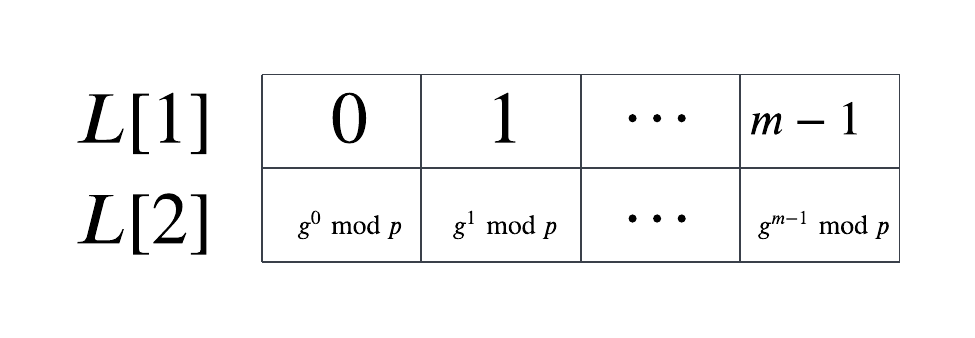
\includegraphics[width=\textwidth]{img/bsgs_L.png}
        \caption{The list $L$ that contains the pre-computed values of $g^{i}$.}
    \end{figure}
    \item The list is ordered by the values. Now, the ordered list will be referred as $L'$. This operation can be executed in $O(m \cdot \operatorname{log}(m) \cdot \operatorname{log}(p))$.
    \item The total cost of the "Baby Steps" part is then $O(m \cdot \operatorname{log}^{2}(p))$.
    \item[\textbf{Giant Steps}] This part consists in finding some $c_0, c_1$ such that $y = c_0 + m \cdot c_1$, given $m = \lceil \sqrt{p} \rceil$. This is done by iterating through the possible values of $c_1$ (\textbf{Giant Steps}), and trying at each iteration to find $c_0$ (\textbf{Baby Steps}).
    \item The first attempt is to find out if $x \in L'[2]$. This is accomplished by using the binary search algorithm, that terminates in $O(\operatorname{log}^{2}(p))$ (The number of iterations is $O(\operatorname{log}(m)) = O(\operatorname{log}(p))$, the comparisons cost $O(\operatorname{log}(p))$ each). If this is verified, then $y$ is the label of the element in $L'[2]$.
    \item The successive attempts try different values for $c_1$ such that:
    \[x \cdot g^{-c_1 \cdot m} \equiv_p g^{i}\]
    Therefore, if $x \cdot g^{-c_1 \cdot m} \in L'[2]$, there must be some $i$ such that $x \equiv_p g^{i + c_1 \cdot m}$. Needless to say, it turns out that $c_0 = i$, that is the label of the found element in $L'[2]$.
    \item The first values for $c_1$ is, trivially, $1$. This means that the first search will be conducted by using $x \cdot g^{-m}$. In order to optimize this, we can use the last value of $L$, that is $g^{m-1}$, and multiply it by $g$, obtaining then $g^m$. At this point, $g^{-m}$ can be found by applying the Extended Euclidean Algorithm.
    \item From this point on, the values of $c_1$ can be obtained by computing $g^{-i \cdot m} = g^{-m} \cdot g^{-(i - 1) \cdot m}$ at each step.
    \item The cost of this part, in the worst case, is $O(m \cdot \operatorname{log}^{2}(p))$, because for $m$ times the Binary search is executed. Fortunately, this formulation of the algorithm can terminate early.
\end{itemize}

\RestyleAlgo{ruled}
\begin{algorithm}
\KwData{$x \in \mathbb{Z}_{p}^{*}, g: <g> = \mathbb{Z}_{p}^{*}$}
\KwResult{$y: g^{y} \equiv_{p} x$}
\caption{Baby-steps/Giant-steps algorithm}\label{alg:baby_steps_giant_steps}
    \Comment{Baby steps part:}
    $c_{0}, c_{1} \gets 0, 0$\;
    $m \gets \lceil \sqrt{p} \rceil$\;
    $G \gets 1$\;
    $L \gets List(m - 1)$\;\Comment{List of $m - 1$ values}
    \For{$c_{i} \in \{0, \dots, m - 1\}$}{
        $G \gets g \cdot G \bmod p$\;
        $L[c_{i}] \gets (c_{i}, G)$\;
    }
    $L' \gets \operatorname{Sort}(L)$\;\Comment{Sorting by the values}
    \Comment{Giant steps part:}
    $G \gets g \cdot G \bmod p$\;\Comment{This is $g^{m} \bmod p$}
    $H \gets \operatorname{EEA}(G, p)$\;\Comment{This is $g^{-m} \bmod p$}
    \If{$x \in L'[2]$}{
        $c_{0} \gets \operatorname{Index}(L', x), 0$\;
        \Return{$c_{0} + c_{1} \cdot m$}\;
    }
    \Else{
        $h \gets x \cdot H$\;
        \For{$c_{1} = \{1, \dots, m - 1\}$}{
            \If{$h \in L'[2]$}{
                $c_{0} \gets \operatorname{Index}(L', x \cdot g^{-c_{1} \cdot m})$\;
                \Return{$c_{0} + c_{1} \cdot m$}\;
            }
            $h \gets h \cdot H \bmod p$\;
        }
    }
\end{algorithm}

\section{Index-Calculus Algorithm}
This algorithm tries to solve the discrete logarithm problem. In order to explain its inner workings, it's necessary to go through the concept of B-smoothness first.
\subsection{B-smoothness test}
The goal of this algorithm is to return $TRUE$ if and only if the input number $n$ is $B$-smooth, given $B$.

\RestyleAlgo{ruled}
\begin{algorithm}
\KwData{$n, B \in \mathbb{Z}$}
\caption{B-smoothness test}\label{alg:b_smoothness_test}
    $P \gets \{p_{i} : p_{i} \text{ is prime} \land p_{i} \leq B\}$\;
    $k \gets |P|$\;
    $N_{1} \gets n$\;
    $V = [0, \dots, 0]$\;
    $i \gets 1$\;
    \Do{$p_{i} \nmid N_{1}$}{\label{b_smt_2}
        \If{$p_{i} \mid N_{1}$}{
            $V[i] \gets V[i+1]$\;
            $N_{1} \gets \frac{N_{1}}{p_{i}}$\;
        }
    }
    \If{$N_{i} = 1$}{
        \Return{$TRUE$}\;
    }
    \If{$N_{1} > 1$}{
        $i \gets i + 1$\;
        \If{$i \leq k$}{
            \GoTo{\ref{b_smt_2}}\;
        }
        \Else{
            \Return{$FALSE$}\;
        }
    }
\end{algorithm}
Let's consider the cost of this algorithm in its worst case.\newline
The worst case is when $\forall i = 1, \dots, k: p_{i} \mid n$. Then
\begin{itemize}
    \item The cost of the division performed on \ref{b_smt_2} is $O(\operatorname{log}^{2}(n))$ b.o.
    \item The length of the loop at \ref{b_smt_2} is $O(\operatorname{log}(n))$, since:
    \[p_{i}^{\alpha_{i}} \leq n \land \alpha_{i} \leq \operatorname{log}(n) \implies \alpha_{i} \leq \frac{\operatorname{log}(n)}{\operatorname{log}(p_{i})}\]
    \item This process is repeated $k = \Pi(B)$ times, that is the number of prime numbers up to $B$.
    \item Therefore, the total cost of this algorithm is $O(\Pi(B) \operatorname{log}^{3}(n))$
\end{itemize}

\subsection{Index-Calculus algorithm}
Let $p$ be a prime number and $g: <g> = \mathbb{Z}_{p}^{*}$. The algorithm proceeds as follows:
\begin{itemize}
    \item[\textbf{Pre-computation}] This part of the algorithm prepares the values that will be used in the following steps of the algorithm.
    \item $B > 0 \in \mathbb{Z}$ is chosen, and the list of the prime numbers up to $B$ is computed. This can be achieved in $O()$ by using the Eratostene's sieve.
    \item $r > 0 \in \mathbb{N}$ is chosen, and $g^r \bmod p$ is computed. Then, if this result is B-smooth, is factorized in prime factors.
    \[g^{r} = p_{1}^{\alpha_{1, r}} \cdot p_{2}^{\alpha_{2, r}} \cdot \dots \cdot p_{k}^{\alpha_{k, r}}\]
    If $g^r \bmod p$ it's not B-smooth the process is repeated with a different $r$. Each attempt has a cost of $O(\operatorname{log}(r) \cdot \operatorname{log}^{2}(p))$. Remark that:
    \begin{align*}
        g^{\operatorname{log}_{g}(p_{i})} &\equiv_{p} p_{i}\\
        \implies r &\equiv_{p} \alpha_{1, r} \cdot \operatorname{log}_{g}(p_{1}) + \dots + \alpha_{k, r} \cdot \operatorname{log}_{g}(p_{k})\\
        \iff g^{r} &\equiv_{p} g^{\sum_{i=1}^{k} \alpha_{i, r} \cdot \operatorname{log}_{g}(p_{i})}
    \end{align*}
    \item This process is repeated $k$ times, in order to obtain the following system:
    \begin{align*}
        \begin{cases}
            r_{1} &\equiv_{p-1} \alpha_{1, r_{1}} \cdot \operatorname{log}_{g}(p_{1}) + \dots + \alpha_{k, r_{1}} \cdot \operatorname{log}_{g}(p_{k})\\
            r_{2} &\equiv_{p-1} \alpha_{1, r_{2}} \cdot \operatorname{log}_{g}(p_{1}) + \dots + \alpha_{k, r_{2}} \cdot \operatorname{log}_{g}(p_{k})\\
            \dots\\
            r_{k} &\equiv_{p-1} \alpha_{1, r_{k}} \cdot \operatorname{log}_{g}(p_{1}) + \dots + \alpha_{k, r_{k}} \cdot \operatorname{log}_{g}(p_{k})\\
        \end{cases}
    \end{align*}
    Consider now $M$, tha matrix of the coefficients $\{\alpha_{i, r_{j}}\}$, where $i,j = 1, \dots, k$. The Chinese Reminder Theorem states that there's a unique solution to this system in $\operatorname{log}_{g}(p_{i})$. This means that $\operatorname{det}(M) \neq 0$, and also $(\operatorname{det}(M), p-1) = 1$.
    \item At this point, we have $g, p, p_{i}, \operatorname{log}_{g}(p_{i})$ for $i = 1, \dots, k$.
    \item[\textbf{Computing DLOG(x)}] This part of the algorithm attemps to find the value of $y$ by using the values that were previously computed.
    \item This step consists in verifying if $x$ is $B$-smooth. That's because, if verified:
    \begin{align*}
        \exists \beta_{i}: x &\equiv_{p} \prod_{i=1}^{k} p_{i}^{\beta_{i}}\\
        \implies g^{y} &\equiv_{p} \prod_{i=1}^{k} g^{\operatorname{log}_{g}(p_{i}) \cdot \beta_{i}}\\
        \implies y &\equiv_{p - 1} \sum_{i=1}^{k} \operatorname{log}_{g}(p_{i}) \cdot \beta_{i}\\
    \end{align*}
    \item In case $x$ is not $B$-smooth, a number $s \in \{1, \dots, p-2\}$ can be generate. Let now be $x_{1} = x \cdot g^{s} \bmod p$. If $x_{1}$ is not $B$-smooth, pick another $s$. If it is, we have that:
    \begin{align*}
        \exists \beta_{i}: x_{1} &\equiv_{p} \prod_{i=1}^{k} p_{i}^{\beta_{i}}\\
        \implies g^{y + s} &\equiv_{p} \prod_{i=1}^{k} g^{\operatorname{log}_{g}(p_{i}) \cdot \beta_{i}}\\
        \implies y + s &\equiv_{p - 1} \sum_{i=1}^{k} \operatorname{log}_{g}(p_{i}) \cdot \beta_{i}\\
    \end{align*}
    Since we generated $s$, we can now easily determine $y$.
\end{itemize}

\section{Pollard's Rho-method for the Discrete Logarithm Problem}
\subsection{General idea}
This algorithm provides a probabilistic solution to the Discrete Logarithm problem, by applying the same idea that is applied to the Factoring Problem.\newline
Consider what follows:
\begin{itemize}
    \item Let $G = <g> = \mathbb{Z}_{p}^{*}$ and $|G| = m \in \mathbb{N}$.
    \item Let also be $x \equiv_{G} g^{y}$, with $y$ unknown.
    \item $G$ is partitioned in 3 subsets, as follows:
    \begin{itemize}
        \item $G_1 = \{a \in \mathbb{Z}_{p}^{*}: 0 < a < \frac{p}{3}\}$
        \item $G_2 = \{a \in \mathbb{Z}_{p}^{*}: \frac{p}{3} \leq a < \frac{2p}{3}\}$
        \item $G_3 = \{a \in \mathbb{Z}_{p}^{*}: \frac{2p}{3} \leq a\}$
    \end{itemize}
    \item Let $f: G \rightarrow G$, such that:
    \begin{align*}
        f(a) &=
        \begin{cases}
            g \cdot a \text{ if } a \in G_1 \\
            a^2 \text{ if } a \in G_2 \\
            x \cdot a \text{ if } a \in G_3 \\
        \end{cases}
    \end{align*}
    \item Consider that $f^{(k)}(a_0) = f \circ f \circ \dots \circ f$, $k$ times. Remark that $a_0 \in G$ is chosen randomly.
    \item The algorithm tries to find some $h, k$ such that $f^{(k)}(a_0) =_{G} f^{(h)}(a_0)$. This is achieved in the same way as the one for the Factoring Problem, by iterating $f(f^{(k - 1)}(a_0))$ and $f(f(f^{(k - 1)}(a_0)))$.
    \item Remark that $\forall k \geq 0, \exists i_{k}, j_{k} \in \mathbb{N}: f^{(k)}(a_0) = x^{i_k} \cdot g^{j_k}$. This is because $a_0 \in G \iff a_0 = g^{j_0}$. Then, we have that:
    \begin{align*}
        (i_{k+1}, j_{k+1}) &=
        \begin{cases}
            (i_{k}, (j_{k} + 1) \bmod m) \cdot a \text{ if } f^{(k)}(a_0) \in G_1 \\
            (2i_{k} \bmod m, 2j_{k} \bmod m) \text{ if } f^{(k)}(a_0) \in G_2 \\
            ((i_{k} + 1) \bmod m, j_{k}) \cdot a \text{ if } f^{(k)}(a_0) \in G_3 \\
        \end{cases}
    \end{align*}
    \item When we find some $f^{(k)}(a_0) = f^{(h)}(a_0)$, we can use this relationship as follows:
    \begin{align*}
        f^{(k)}(a_0) &= f^{(h)}(a_0)\\
        x^{i_k} \cdot g^{j_k} &=_G x^{i_h} \cdot g^{j_h}\\
        g^{j_k - j_h} &=_G x^{i_k - j_h} =_G g^{y \cdot (i_k - i_h)}\\
        j_k - j_h &\equiv_{m} y \cdot (i_k - i_h)\\
        \text{If } (i_k - i_h, m) = 1 \text{ then, } y \equiv_{m} (j_k - j_h) \cdot (i_k - i_h)^{-1}\\
        \text{If } (i_k - i_h, m) = d > 1 \text{ then, } y \cdot (i_k - i_h) \equiv_{m} (j_k - j_h)\\
        \text{Reduced congruence:}\\
        y \cdot (\frac{i_k - i_h}{d}) &= (\frac{j_k - j_h}{d}) \bmod \frac{m}{d}\\
        \implies (\frac{i_k - i_h}{d}, \frac{m}{d}) &= 1\\
        \text{Therefore, } y &= (\frac{j_k - j_h}{d}) \cdot (\frac{i_k - i_h}{d}) \bmod \frac{m}{d}
    \end{align*}
    At this point, verify that $g^y \equiv_m x$. If it doesn't work, try:
    \[g^{y + \mathcal{l} \cdot (\frac{m}{d}), \text{ where } \mathcal{l} \in \{0, 1, \dots, d - 1\}}\]
\end{itemize}

\subsection{Floyd's iteration}
This method, as its correspondant for the Factoring Problem, aims to optimize the research for the collisions.
\begin{itemize}
    \item Assume that you have found some $m_0 < l_0$ such that $f^{(m_0)}(a_0) = f^{(l_0)}(a_0)$. Then, let $\mu = l_0 - m_0$.
    \item Then, you'll have that $f^{(m)}(a_0) = f^{(l)}(a_0) \implies l \equiv_{\mu} m$.
    \item Let now $z = \mu \cdot \lceil \frac{m_0}{\mu} \rceil$ and let $2z = z + \mu \cdot \lceil \frac{m_0}{\mu} \rceil$. Then $f^{(z)}(a_0) = f^{(2z)}(a_0)$.
    \item Let now $H_{1}(s) = f^{(s)}(a_0)$, $H_{2}(s) = f^{(2s)}(a_0)$ and
    $H_{1}(s + 1) = f(H_{1}(s))$, $H_{2}(s + 1) = f(f(H_{2}(s)))$
    \item This allows to spare some computation steps, since we're only looking for meaningful collisions after we've found the first one. This means that we must perform only $O(\sqrt{m})$ steps in order to have a probability of $\frac{1}{2}$ to find $y$.
\end{itemize}

\section{Chaum-van Heijst-Pfitzmann compression function}
Consider the following:
\begin{itemize}
    \item Let $p, q$ be two prime numbers such that $p \equiv 3 \bmod 4$ and $q = \frac{p-1}{2}$.
    \item Let $<g> = \mathbb{Z}_{p}^{*}$, and $t \in \mathbb{Z}_{p}^{*}$.
\end{itemize}
The hash function $h$ is defined as
\begin{align*}
    h: \mathbb{Z}_{q} \times \mathbb{Z}_{q} &\rightarrow \mathbb{Z}_{p}^{*}\\
    h(a, b) &= g^{a} \cdot t^{b} \bmod p
\end{align*}
The signature of the cleary states that the input's size is reduced of a factor 2. Let's see why:
\begin{align*}
    \operatorname{Size}((a,b)) &= 2 \cdot \operatorname{log}(q)\\
    = 2 \cdot \operatorname{log}(\frac{p-1}{2}) &= 2 \cdot (\operatorname{log}(p-1) - \operatorname{log}(2))\\
    &= 2 \cdot \operatorname{log}(p \cdot (1 - \frac{1}{p})) - 2 \cdot \operatorname{log}(2)\\
    &= 2 \cdot \operatorname{log}(p) + 2 \cdot \operatorname{log}(1 - \frac{1}{p})) - 2 \cdot \operatorname{log}(2)\\
    &= 2 \cdot \operatorname{log}(p) - 2 \cdot \operatorname{log}(2) + O(\frac{1}{p}) \text{, Since } \operatorname{log}(1 - \frac{1}{p}) = O(\frac{1}{p})
\end{align*}
Therefore, $\operatorname{Size}((a,b))$ is approximately twice the size of the output, that is $O(\operatorname{log}(p))$.\newline
What follows is the proof that the security of this hash function stands on the hardness of the Discrete Logarithm Problem.
\begin{itemize}
    \item
\end{itemize}


\chapter*{Useful Facts}
\begin{itemize}
    \item The \href{https://gmplib.org/}{GMP library} is a free library for arbitrary precision arithmetic. It implements all the basic arithmetic operations with the maximum efficency possible.
\end{itemize}

\listofalgorithms
\listoftheorems[ignoreall, show={theorem}]

\begingroup               % Temporarily disable \clearpage to show both lists on one page
  \let\clearpage\relax    % http://tex.stackexchange.com/a/14511/104449
  \renewcommand{\listtheoremname}{List of Lemmas}
  \listoftheorems[ignoreall, show={lemma}]
\endgroup

\end{document}
